% Template visuel repris depuis TFIDF/presentation/main.tex.
% Presentation: TF-IDF et explicabilite des modeles.
\documentclass[10pt]{beamer}
\usepackage[utf8]{inputenc}
% Le template original charge xeCJK. On le garde seulement si sa dependance
% locale est disponible, afin que la presentation compile aussi sans support CJK.
\IfFileExists{ctexhook.sty}{\usepackage{xeCJK}}{}
\usepackage{graphicx}
\IfFileExists{mathtools.sty}{\usepackage{mathtools}}{}
\IfFileExists{utopia.sty}{\usepackage{utopia}}{}
\usetheme{CambridgeUS}
\usecolortheme{dolphin}
\usepackage{tcolorbox}
\IfFileExists{tabularray.sty}{\usepackage{tabularray}}{}
\IfFileExists{float.sty}{\usepackage{float}}{}
\IfFileExists{adjustbox.sty}{\usepackage{adjustbox}}{}
\IfFileExists{caption.sty}{\usepackage{caption}}{}
\IfFileExists{subcaption.sty}{\usepackage{subcaption}}{}
\IfFileExists{multirow.sty}{\usepackage{multirow}}{}
\usepackage{tikz}
\IfFileExists{booktabs.sty}{\usepackage{booktabs}}{%
    \newcommand{\toprule}{\hline}
    \newcommand{\midrule}{\hline}
    \newcommand{\bottomrule}{\hline}
}
\IfFileExists{makecell.sty}{\usepackage{makecell}}{}
\usepackage{array}
\usepackage{longtable}
\IfFileExists{natbib.sty}{\usepackage{natbib}}{}
\usepackage{hyperref}
\providecommand\theadfont{}
\renewcommand\theadfont{\bfseries}

\usetikzlibrary{positioning}
\usetikzlibrary{calc}
\usetikzlibrary{arrows.meta}
\usetikzlibrary{shapes}
\usetikzlibrary{shapes.geometric}

% Palette conservee depuis le template original.
\definecolor{lightred}{RGB}{180,227,236}
\definecolor{middlelightred}{RGB}{138,22,57}
\definecolor{middledered}{RGB}{217,79,120}
\definecolor{redforsnnu}{RGB}{176,44,89}
\definecolor{darkred}{RGB}{138,22,57}

\setbeamercolor*{palette primary}{bg=redforsnnu, fg=white}
\setbeamercolor*{palette secondary}{bg=middledered, fg=white}
\setbeamercolor*{palette tertiary}{bg=middlelightred, fg=white}
\setbeamercolor*{titlelike}{fg=redforsnnu}
\setbeamercolor*{title}{bg=darkred, fg=white}
\setbeamercolor*{item}{fg=redforsnnu}
\setbeamercolor*{caption name}{fg=middledered}

\usefonttheme{professionalfonts}

% Affiche une vraie figure si elle existe, sinon un placeholder compilable.
% Remplacer progressivement les chemins par des exports propres dans figures/*.pdf.
\newcommand{\safegraphic}[2][0.85\linewidth]{%
    \IfFileExists{#2}{%
        \includegraphics[width=#1]{#2}%
    }{%
        \begin{tcolorbox}[width=#1, colback=lightred!20, colframe=redforsnnu, title=Figure a completer]
            \centering
            \scriptsize
            Placeholder pour la figure attendue.\\[0.15cm]
            {\tiny\url{#2}}
        \end{tcolorbox}%
    }%
}

\newcommand{\safegraphicfit}[3][0.85\linewidth]{%
    \IfFileExists{#3}{%
        \includegraphics[width=#1,height=#2,keepaspectratio]{#3}%
    }{%
        \begin{tcolorbox}[width=#1, colback=lightred!20, colframe=redforsnnu, title=Figure a completer]
            \centering
            \scriptsize
            Placeholder pour la figure attendue.\\[0.15cm]
            {\tiny\url{#3}}
        \end{tcolorbox}%
    }%
}

\newcommand{\highlight}[1]{\textcolor{redforsnnu}{\textbf{#1}}}

\titlegraphic{
\begin{tikzpicture}[overlay, remember picture]
    \node[anchor=north, yshift=-0.7cm] at (current page.north){
        \begin{minipage}{\textwidth}
            \centering
            \IfFileExists{images/logo.png}{%
                
\includegraphics[height=1.7cm]{images/logo.png}%
            }{%
                \IfFileExists{images/logo.jpg}{%
                    
\includegraphics[height=1.7cm]{images/logo.jpg}%
                }{%
                    \vspace{0.2cm}
                    {\small Universite Paris Cite}
                }%
            }
        \end{minipage}
    };
\end{tikzpicture}
}

\setbeamerfont{title}{size=\large}
\setbeamerfont{subtitle}{size=\small}
\setbeamerfont{author}{size=\small}
\setbeamerfont{date}{size=\small}
\setbeamerfont{institute}{size=\scriptsize}

\title[]{Explicabilité des modèles de classification de textes,\\ application NLP -- Approche TF-IDF}
\subtitle{}
\author[]{\textbf{Hamza OMARI}}
\institute[]{Modélisation des systèmes intelligents\\Master 2 vision et machine intelligente}
\date[\textcolor{white}{2026}]{2026}

\AtBeginSection[]{
  \begin{frame}
  \vfill
  \transfade
  \centering
  \begin{beamercolorbox}[sep=8pt,center,shadow=true,rounded=true]{title}
    \usebeamerfont{title}\insertsectionhead\par%
  \end{beamercolorbox}
  \vfill
  \end{frame}
}

\begin{document}

\begin{frame}[plain]
    \inserttitlegraphic
    \vspace*{2.35cm}
    \begin{center}
        \begin{beamercolorbox}[sep=8pt,center,shadow=true,rounded=true]{title}
            \usebeamerfont{title}\inserttitle\par
        \end{beamercolorbox}
        \vspace{0.45cm}
        {\usebeamerfont{author}\insertauthor\par}
        \vspace{0.25cm}
        {\usebeamerfont{institute}\insertinstitute\par}
        \vspace{0.35cm}
        {\usebeamerfont{date}\insertdate\par}
    \end{center}
\end{frame}

\begin{frame}{Table of Contents}
    \tableofcontents
\end{frame}

%------------------------------------------------------------
\section{Contexte}
%------------------------------------------------------------

\begin{frame}{Probleme et objectif}
    \vspace{-0.15cm}
    \begin{itemize}\scriptsize
        \item Construire un classifieur TF-IDF + MLP pour la prediction \texttt{homme}/\texttt{femme}.
        \item Expliquer les decisions du modele avec Integrated Gradients, LRP et les tests de perturbation.
    \end{itemize}
    \vspace{0.02cm}
    \centering
    \safegraphicfit[0.97\linewidth]{0.66\textheight}{images/overview.png}
\end{frame}

\begin{frame}{Dataset}
    \vspace{-0.2cm}
    \begin{columns}[T,onlytextwidth]
        \begin{column}{0.40\textwidth}
            \begin{tcolorbox}[colback=lightred!20, colframe=redforsnnu, title=Taille des splits]
                \tiny
                \begin{center}
                \setlength{\tabcolsep}{2pt}
                \begin{tabular}{@{}lrrr@{}}
                    \toprule
                    Split & Total & Femme & Homme \\
                    \midrule
                    Train & 852 & 492 & 360 \\
                    Val. & 284 & 164 & 120 \\
                    Test & 285 & 165 & 120 \\
                    \bottomrule
                \end{tabular}
                \end{center}
            \end{tcolorbox}
            \begin{itemize}\small
                \item Les labels sont extraits des noms de fichiers.
                \item Les distributions sont proches entre validation et test.
                \item Risque: biais possibles dans les donnees et dans le protocole de labellisation.
            \end{itemize}
        \end{column}
        \begin{column}{0.52\textwidth}
            \centering
            \vspace{-0.12cm}
            \begin{minipage}{\linewidth}
                \centering
                \safegraphicfit[0.78\linewidth]{0.24\textheight}{images/distribution_total.png}\\[-0.02cm]
                {\tiny Distribution totale homme/femme\par}
            \end{minipage}

            \vspace{0.08cm}
            \begin{minipage}{\linewidth}
                \centering
                \safegraphicfit[0.78\linewidth]{0.24\textheight}{images/distribution_splits.png}\\[-0.02cm]
                {\tiny Distribution des classes par split\par}
            \end{minipage}
        \end{column}
    \end{columns}
\end{frame}

\begin{frame}{Pipeline global}
    \begin{figure}
    \centering
    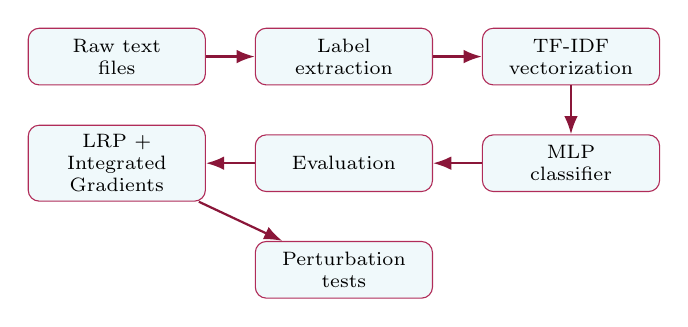
\begin{tikzpicture}[
        node distance=0.62cm,
        box/.style={draw=redforsnnu, rounded corners, fill=lightred!20,
                    minimum width=2.25cm, minimum height=0.72cm,
                    align=center, font=\scriptsize},
        arrow/.style={-Latex, thick, draw=darkred}
    ]
        \node[box] (raw) {Raw text\\files};
        \node[box, right=of raw] (labels) {Label\\extraction};
        \node[box, right=of labels] (tfidf) {TF-IDF\\vectorization};
        \node[box, below=of tfidf] (mlp) {MLP\\classifier};
        \node[box, left=of mlp] (eval) {Evaluation};
        \node[box, left=of eval] (xai) {LRP +\\Integrated\\Gradients};
        \node[box, below=of eval] (pert) {Perturbation\\tests};

        \draw[arrow] (raw) -- (labels);
        \draw[arrow] (labels) -- (tfidf);
        \draw[arrow] (tfidf) -- (mlp);
        \draw[arrow] (mlp) -- (eval);
        \draw[arrow] (eval) -- (xai);
        \draw[arrow] (xai) -- (pert);
    \end{tikzpicture}
    \end{figure}

\end{frame}

%------------------------------------------------------------
\section{Architecture du classifieur}
%------------------------------------------------------------

\begin{frame}{Architecture 1}
    \centering
    \safegraphicfit[0.96\linewidth]{0.74\textheight}{images/architecture_1.png}
\end{frame}

\begin{frame}{Courbes d'entrainement -- architecture 1}
    \begin{tcolorbox}[colback=lightred!20, colframe=redforsnnu, title=Hyperparametres]
        \scriptsize
        \begin{tabular}{@{}lll@{\hspace{0.6cm}}lll@{}}
            \texttt{BATCH\_SIZE} & = & 8 &
            \texttt{EPOCHS} & = & 50 \\
            Optimizer & = & AdamW &
            \texttt{LEARNING\_RATE} & = & \texttt{1e-4} \\
            \texttt{WEIGHT\_DECAY} & = & \texttt{1e-4} &
            & &
        \end{tabular}
    \end{tcolorbox}
    \vspace{0.05cm}
    \centering
    \safegraphicfit[0.78\linewidth]{0.47\textheight}{../vis/tfidf_loss_curve.png}
\end{frame}

\begin{frame}{Architecture pour reduire l'overfitting}
    \centering
    \safegraphicfit[0.96\linewidth]{0.74\textheight}{images/architecture_2_clean.png}
\end{frame}

\begin{frame}{Nouvelles courbes d'entrainement}
    \centering
    \safegraphic[0.82\linewidth]{images/nouvelle_courbe_loss.png}
\end{frame}

%------------------------------------------------------------
\section{Evaluation}
%------------------------------------------------------------

\begin{frame}{Resultats de classification}
    \begin{columns}[T]
        \begin{column}{0.45\textwidth}
            \begin{tcolorbox}[colback=lightred!20, colframe=redforsnnu, title=Metriques globales]
                \begin{itemize}\small
                    \item Accuracy test: \highlight{0.853}
                    \item Macro F1: \highlight{0.850}
                    \item Weighted F1: \highlight{0.853}
                \end{itemize}
            \end{tcolorbox}
            \begin{center}
            \scriptsize
            \begin{tabular}{lccc}
                \toprule
                Classe & Precision & Recall & F1 \\
                \midrule
                Femme & 0.882 & 0.861 & 0.871 \\
                Homme & 0.815 & 0.842 & 0.828 \\
                \bottomrule
            \end{tabular}
            \end{center}
        \end{column}
        \begin{column}{0.50\textwidth}
            \begin{figure}
                \centering
                \safegraphic[0.9\linewidth]{images/matrice_confusion.png}
            \end{figure}
        \end{column}
    \end{columns}
    \vspace{0.1cm}
    \centering
    \small Le coeur de l'etude n'est pas seulement la performance, mais l'explication de cette performance.
\end{frame}

%------------------------------------------------------------
\section{Explicabilite}
%------------------------------------------------------------

\begin{frame}{Integrated Gradients}
    \centering
    \vfill
    {\small\textbf{Principe de la methode Integrated Gradients}\par}
    \vspace{0.08cm}
    \makebox[\textwidth][c]{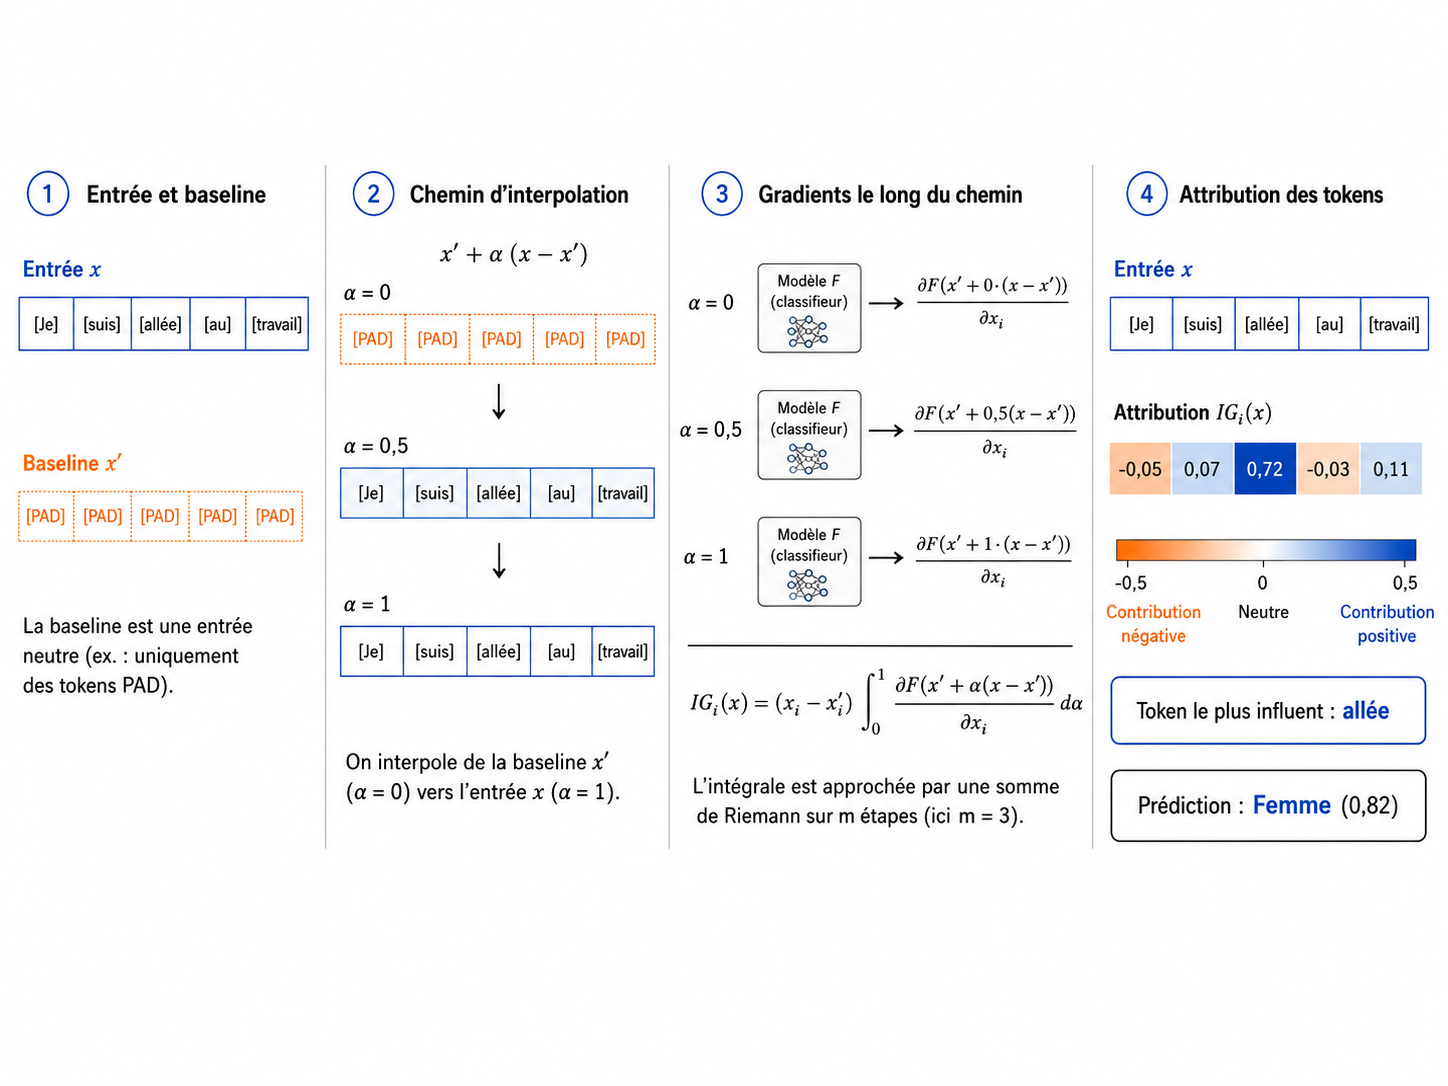
\includegraphics[width=0.88\textwidth,height=0.64\textheight,keepaspectratio]{images/integrated_gradients.png}}
    \vspace{0.08cm}
    {\tiny image générée par IA, prompt engineering.\par}
    \vfill
\end{frame}

\begin{frame}{LRP}
    \centering
    \vfill
    {\small\textbf{Principe de la methode LRP}\par}
    \vspace{0.08cm}
    \makebox[\textwidth][c]{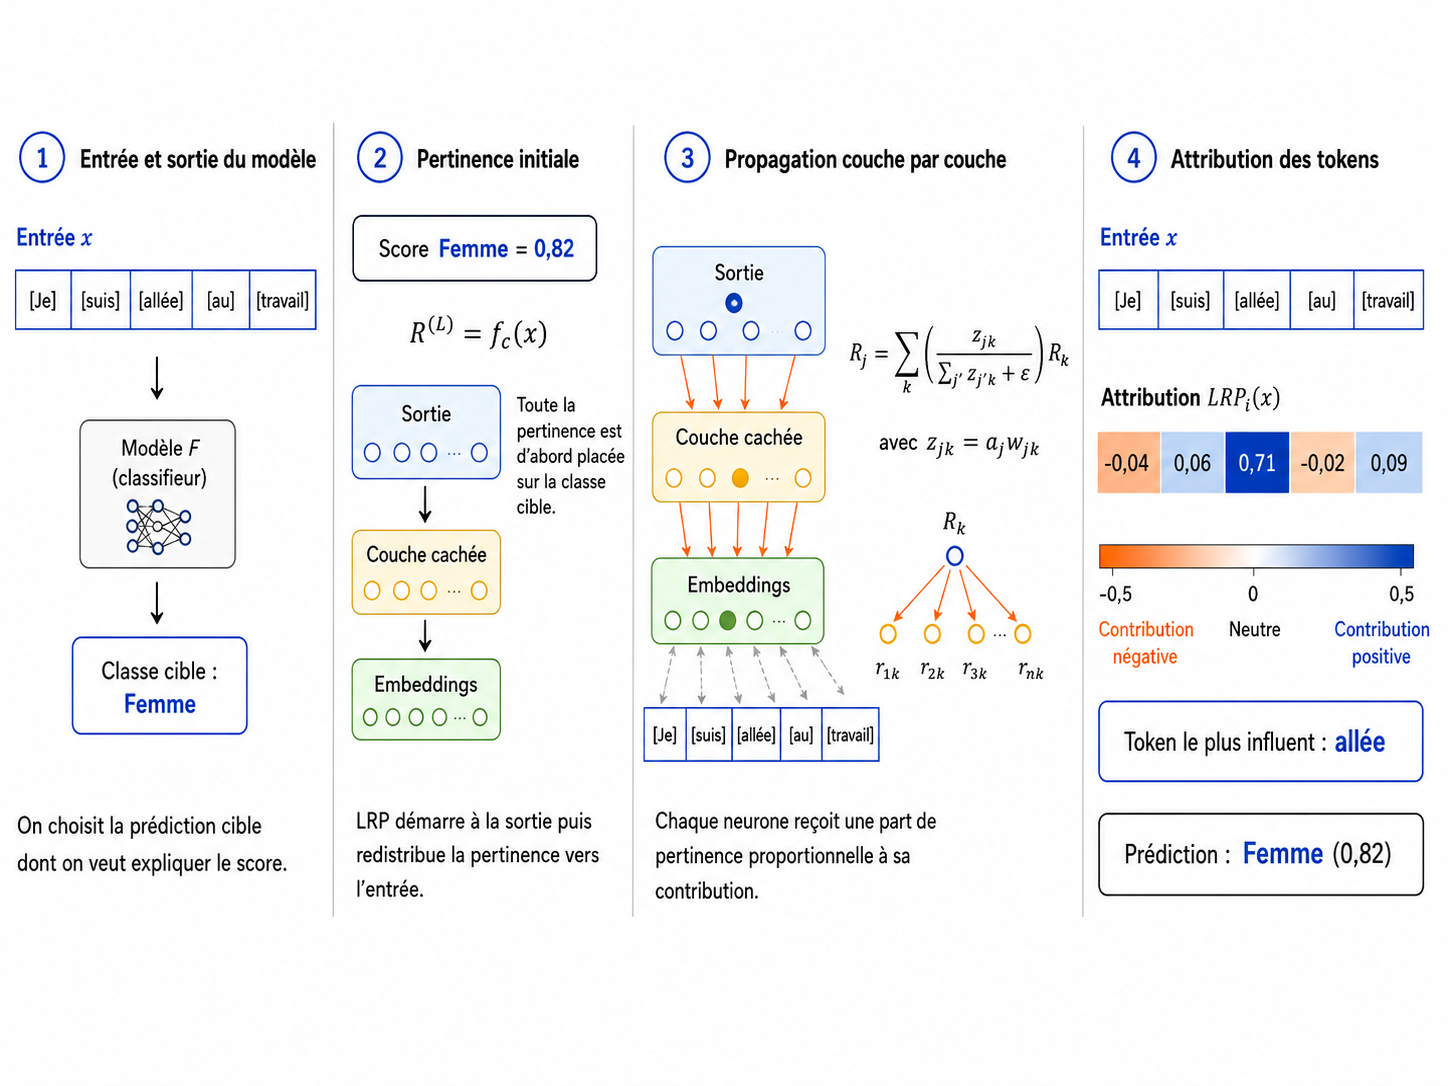
\includegraphics[width=0.88\textwidth,height=0.64\textheight,keepaspectratio]{images/LRP.png}}
    \vspace{0.08cm}
    {\tiny image générée par IA, prompt engineering.\par}
    \vfill
\end{frame}

\begin{frame}{Explications globales: Integrated Gradients}
    \begin{columns}[T]
        \begin{column}{0.49\textwidth}
            \centering
            % TODO: eventuellement exporter vers figures/ig_top_terms_homme.pdf.
            \safegraphic[0.98\linewidth]{../vis/tfidf_ig_top_homme_terms.png}
            {\centering\scriptsize Termes soutenant les predictions \texttt{homme}\par}
        \end{column}
        \begin{column}{0.49\textwidth}
            \centering
            % TODO: eventuellement exporter vers figures/ig_top_terms_femme.pdf.
            \safegraphic[0.98\linewidth]{../vis/tfidf_ig_top_femme_terms.png}
            {\centering\scriptsize Termes soutenant les predictions \texttt{femme}\par}
        \end{column}
    \end{columns}
    \vspace{0.1cm}
    \centering
    \scriptsize Formulation volontaire: ces termes soutiennent le modele, ils ne definissent pas des groupes humains.
\end{frame}

\begin{frame}{Explications globales: LRP}
    \begin{columns}[T]
        \begin{column}{0.49\textwidth}
            \centering
            % TODO: eventuellement exporter vers figures/lrp_top_terms_homme.pdf.
            \safegraphic[0.98\linewidth]{../vis/tfidf_lrp_top_homme_terms.png}
            {\centering\scriptsize Termes soutenant les predictions \texttt{homme}\par}
        \end{column}
        \begin{column}{0.49\textwidth}
            \centering
            % TODO: eventuellement exporter vers figures/lrp_top_terms_femme.pdf.
            \safegraphic[0.98\linewidth]{../vis/tfidf_lrp_top_femme_terms.png}
            {\centering\scriptsize Termes soutenant les predictions \texttt{femme}\par}
        \end{column}
    \end{columns}
    \vspace{0.1cm}
    \centering
    \scriptsize LRP propage la relevance a travers le reseau; BatchNorm/Dropout sont traites comme pass-through.
\end{frame}

\begin{frame}{Convergence des attributions IG et LRP}
    \vspace{0.45cm}
    \begin{center}
        \scriptsize
        \begin{tabular}{ll}
            \toprule
            Classe & Termes communs IG/LRP \\
            \midrule
            Homme & fit, jules \\
            Femme & marie, fanny, tante \\
            \bottomrule
        \end{tabular}
    \end{center}

    \vspace{0.35cm}
    \begin{center}
        \small
        \begin{minipage}{0.92\textwidth}
            \raggedright
            L'intersection entre IG et LRP permet d'identifier les termes les plus stables pour chaque classe.

            \vspace{0.12cm}
            Les termes communs montrent que les deux méthodes convergent partiellement vers les mêmes indices lexicaux.
        \end{minipage}
    \end{center}
\end{frame}

\begin{frame}{Visualisation des scores d'attribution}
    \centering
    \small Les scores d'attribution sont visualises directement sur le texte pour relier les termes aux decisions du modele.
    \vspace{0.2cm}

    \safegraphic[0.88\linewidth]{images/example_viz_score.png}
\end{frame}

%------------------------------------------------------------
\section{Perturbations}
%------------------------------------------------------------

\begin{frame}{Protocole de perturbation}
    \begin{columns}[T]
        \begin{column}{0.50\textwidth}
            \begin{tcolorbox}[colback=lightred!20, colframe=redforsnnu, title=Validation comportementale]
                \begin{enumerate}\small
                    \item Selectionner des textes correctement classes.
                    \item Recuperer les top termes explicatifs.
                    \item Perturber les textes.
                    \item Relancer le modele.
                    \item Mesurer l'impact.
                \end{enumerate}
            \end{tcolorbox}
        \end{column}
        \begin{column}{0.45\textwidth}
            \begin{tcolorbox}[colback=middledered!20, colframe=darkred, title=Modes testes]
                \begin{itemize}\small
                    \item \texttt{remove}: suppression des termes.
                    \item \texttt{mask}: remplacement par \texttt{[MASK]}.
                    \item \texttt{swap}: remplacement par des termes de l'autre classe.
                \end{itemize}
            \end{tcolorbox}
        \end{column}
    \end{columns}

    \vspace{0.2cm}
    \centering
    \small Mesures: baisse d'accuracy, baisse de confiance, nombre de predictions inversees.
\end{frame}

\begin{frame}{Perturbations: accuracy et confiance}
    \begin{columns}[T]
        \begin{column}{0.49\textwidth}
            \centering
            \safegraphic[0.98\linewidth]{../vis_old/tfidf_perturbation_accuracy_drop.png}
            {\centering\scriptsize Accuracy avant/apres perturbation\par}
        \end{column}
        \begin{column}{0.49\textwidth}
            \centering
            \safegraphic[0.98\linewidth]{../vis_old/tfidf_perturbation_confidence_drop.png}
            {\centering\scriptsize Confidence drop\par}
        \end{column}
    \end{columns}
\end{frame}

\begin{frame}{Resultats des perturbations}
    \vspace{-0.25cm}
    \begin{center}
    \scriptsize
    \begin{tabular}{llccc}
        \toprule
        Methode & Mode & Acc. apres & Baisse acc. & Predictions inversees \\
        \midrule
        IG & remove & 0.97 & 0.03 & 3 \\
        IG & mask & 0.97 & 0.03 & 3 \\
        IG & swap & 0.90 & 0.10 & 10 \\
        LRP & remove & 1.00 & 0.00 & 0 \\
        LRP & mask & 1.00 & 0.00 & 0 \\
        LRP & swap & 0.97 & 0.03 & 3 \\
        Intersection & remove & 0.99 & 0.01 & 1 \\
        Intersection & mask & 0.99 & 0.01 & 1 \\
        Intersection & swap & 0.98 & 0.02 & 2 \\
        \bottomrule
    \end{tabular}
    \end{center}
    \vspace{0.1cm}
    \begin{itemize}\small
        \item Si la suppression ou modification des termes explicatifs reduit l'accuracy ou la confiance,
        alors ces termes sont comportementalement importants pour ce modele.
    \end{itemize}
\end{frame}

%------------------------------------------------------------
\section{Limites et conclusion}
%------------------------------------------------------------

\begin{frame}{Limites}
    \begin{columns}[T]
        \begin{column}{0.48\textwidth}
            \begin{tcolorbox}[colback=lightred!20, colframe=redforsnnu, title=Representation et donnees]
                \begin{itemize}\small
                    \item TF-IDF ignore l'ordre des mots et la syntaxe.
                    \item Les labels et les textes peuvent contenir des biais.
                    \item Les resultats dependent de ce corpus.
                \end{itemize}
            \end{tcolorbox}
        \end{column}
        \begin{column}{0.48\textwidth}
            \begin{tcolorbox}[colback=middledered!20, colframe=darkred, title=Explicabilite]
                \begin{itemize}\small
                    \item Les explications sont specifiques au modele.
                    \item Les perturbations peuvent creer des textes peu naturels.
                    \item LRP a travers BatchNorm/Dropout est approxime comme pass-through.
                \end{itemize}
            \end{tcolorbox}
        \end{column}
    \end{columns}
    \vspace{0.2cm}
    \centering
    \small Aucune conclusion ne doit etre lue comme un marqueur universel du genre.
\end{frame}

\begin{frame}{Conclusion}
    \begin{tcolorbox}[colback=lightred!20, colframe=redforsnnu, title=Messages a retenir]
        \begin{enumerate}\small
            \item TF-IDF + MLP donne une baseline forte et interpretable.
            \item Integrated Gradients et LRP identifient les termes qui influencent les predictions.
            \item Les perturbations verifient si ces termes affectent reellement le comportement du modele.
            \item On explique ce classifieur sur ce dataset, pas le langage humain en general.
        \end{enumerate}
    \end{tcolorbox}
\end{frame}

\begin{frame}[plain]
    \centering
    \vfill
    {\Large\textbf{Merci pour votre attention}\par}
    \vspace{0.8cm}
    {\Huge\textbf{Questions ?}\par}
    \vfill
\end{frame}

\end{document}
